\documentclass[aps,prb,twocolumn,superscriptaddress,floatfix,nofootinbib]{revtex4-2}

\usepackage{amsmath}
\usepackage{amssymb}
\usepackage{graphicx}
\usepackage[colorlinks=true,linkcolor=blue,citecolor=blue,urlcolor=blue]{hyperref}

\begin{document}

\title{Which electrical axes separate intrinsic from extrinsic fractional
       Shapiro steps, and which do not}

\author{Faruk Sami Bilgin}
\email{fsamibilgin@gmail.com}
\affiliation{Independent researcher}

\date{\today}

\begin{abstract}
Half-integer and other fractional Shapiro steps are attributed either to a second
harmonic in the current--phase relation or to trapped flux, and the standard way
of separating the two is a battery of tests that all perturb the sample. We ask
which purely electrical axes discriminate, simulating a two-harmonic junction
against an asymmetric inductive two-link loop in a current-biased frame. Two
axes do not. The drive-frequency trend's sign is not diagnostic: the loop
reproduces either direction depending on its screening parameter, from $-61\%$
at $\beta_L=4$ to $+647\%$ at $100$, against a uniform $+56\%$ to $+102\%$ for
the intrinsic mechanism. Initial-condition sensitivity vanishes at all but one
of the settings scanned. A third axis works, but conditionally, and saying so
precisely is most of what this paper contributes. The half-step width has a node
in drive amplitude, pinned for the intrinsic mechanism by the published
$|J_1(2\alpha)|$ envelope at $\alpha=j_{1,1}/2=1.9159$ and found here at
$1.92$--$1.94$ across a $2.7$-fold range of harmonic content, with node depths
three orders below the curve's peak. The loop's node is displaced, but by an
amount that runs from $+9.6\%$ to $+22.1\%$ and then \emph{saturates}, so it
cannot be inverted to measure the inductance; and below Frolov's existence
threshold $\beta_L>2a/(1-a^2)=0.659$ the loop has no half step to have a node,
which is the regime in which published perturbation theory puts its node at
$1.9159$ too. A fourth axis, trapped flux, does not separate intrinsic from
extrinsic but separates the two published extrinsic channels: the loop's half
step requires frustration, peaking at $f=0.50$--$0.60$ and absent at integer
flux, where the alternating-$j_c$ channel's is finite. Finally we report, and do
not resolve, a systematic that prevents a thermal-scaling verdict: the control
subtraction the method relies on does not cancel, because the two
current--phase relations do not share the ohmic slope that sets the estimator's
floor, and the residual is $1.5\%$ of the half-step net width but $59\%$ of the
quarter-step one.
\end{abstract}

\maketitle

\section{Introduction}

A Josephson junction under microwave drive locks its average voltage to
$V=(n/k)\,\hbar\omega/2e$. Steps with $k=1$ follow from any current--phase
relation (CPR); steps with $k>1$ do not, and their appearance is routinely read
as evidence about the junction. In the \emph{intrinsic} reading the CPR carries
a second harmonic and the fractional steps fingerprint the pairing. In the
\emph{extrinsic} reading the junction is spatially inhomogeneous --- trapped
flux, a vortex, an unintended parallel path --- and they say nothing about it.

Zhu \emph{et al.}~\cite{Zhu2026} measured half-integer and odd-denominator steps
in twisted cuprate junctions and assigned them to trapped vortices. Their
evidence was operational and it works: the steps vanished on thermal cycling and
returned after small-field or large-current training. The extrinsic reading
itself is older --- Early \emph{et al.}~\cite{Early1994} established parallel
junctions within high-$T_c$ grain boundaries, and Terpstra \emph{et
al.}~\cite{Terpstra1995} reported odd-denominator steps from synchronised vortex
motion in a wide junction --- and Zhu \emph{et al.} note that Bi-2212's
Josephson penetration depth, below $1\,\mu$m, is smaller than their junction
overlap, so parallel paths are intrinsically likely.

Every test in that battery perturbs the sample. The question here is whether the
electrical measurement an experiment already performs, a Shapiro map, contains
an axis along which the two mechanisms differ. We find that two natural
candidates do not, that one does within a bounded parameter range, and that a
fourth separates something else worth separating. We also report a measurement
we could not complete honestly, and why.

\section{Models and method}

Time is reduced as $\tau=\omega_c t$, currents are in units of $I_c$, the
reduced voltage is $v=\langle\dot\phi\rangle$, and the reduced drive amplitude
is $\alpha=i_{\rm ac}/\Omega$, the amplitude of the phase modulation the drive
imposes. Steps sit at $v=(n/k)\Omega$.

The intrinsic model is the overdamped two-harmonic junction,
\begin{equation}
  \dot\phi = i_{\rm dc} + i_{\rm ac}\cos\Omega\tau
             - \left[c_1\sin\phi + c_2\sin 2\phi\right] + \eta ,
  \label{eq:intrinsic}
\end{equation}
whose fractional step amplitudes Tsarev and Fominov~\cite{Tsarev2025} give in
closed form. Where a specific harmonic content is needed we use the
short-junction Beenakker CPR~\cite{Beenakker1991} at transparency $0.8$.

The extrinsic model is two parallel weak links sharing a loop,
\begin{align}
  \dot\phi_1 &= i_b - 2 j_{\rm circ} - 2a_1\sin\phi_1 + \eta_1 ,\nonumber\\
  \dot\phi_2 &= i_b + 2 j_{\rm circ} - 2a_2\sin\phi_2 + \eta_2 ,
  \label{eq:extrinsic}\\
  j_{\rm circ} &= \left[(\phi_1-\phi_2) - 2\pi f\right]/\beta_L ,\nonumber
\end{align}
with $f$ the trapped flux in units of $\Phi_0$,
$\beta_L = 2\pi L I_c/\Phi_0$, and $a_1+a_2=1$ setting the asymmetry, fixed at
$a=0.3$ throughout. No harmonic is put in by hand. This model is not new: it is
that of Frolov \emph{et al.}~\cite{Frolov2006}, and Mori and
Maekawa~\cite{Mori2021} solve the same equations perturbatively, showing that to
first order in $\beta_L$ the loop reduces to a two-harmonic CPR. Frolov
\emph{et al.} also give the existence condition for the spontaneous circulating
current that produces the half step, $\beta_L > 2a/(1-a^2)$, which is $0.659$ at
$a=0.3$; it matters below.

Widths are measured with a Gaussian transit estimator,
\begin{equation}
  w = \int \! di_{\rm dc}\,
      \exp\!\left[-\frac{(v(i_{\rm dc})-v_{\rm step})^2}{2\sigma_k^2}\right] ,
  \label{eq:kernel}
\end{equation}
$\sigma_k=0.025$, on an absolute current grid. On a linear transit
Eq.~\eqref{eq:kernel} returns $\sigma_k\sqrt{2\pi}/|dv/di|$, which we reproduce
to $2\times10^{-16}$. Widths are quoted \emph{net} of a control: for the
intrinsic model the same estimator evaluated for a sinusoidal CPR, and for the
loop the same estimator at $f=0$, where an unfrustrated loop has no half step.
The two controls are different objects, which Sec.~\ref{sec:node} keeps in
view. Section~\ref{sec:fails} is the exception: those numbers predate the
kernel estimator and were measured by counting grid points inside the plateau,
which quantises the width in units of the bias step; the $\pm10\%$ sensitivity
we find on refining that step is an unremoved systematic there.

\section{Two axes that do not discriminate}
\label{sec:fails}

\paragraph*{Drive frequency.} The intrinsic mechanism raises $w_{1/2}/w_1$ as
the drive frequency rises from $\Omega=2$ to $8$, by $+56\%$ to $+102\%$ across
a range of $c_2/c_1$. The loop can do either: $+31\%$ at $\beta_L=0.5$, $-61\%$
at $4$, $+279\%$ at $30$, $+647\%$ at $100$. The sign carries no information.
What survives is a one-sided exclusion --- a measured increase below $56\%$
cannot come from the intrinsic mechanism in this range of harmonic content ---
carrying the grid systematic noted above.

\paragraph*{Initial conditions.} Equation~\eqref{eq:extrinsic} has two dynamical
variables and could support multistability, whose signature would be hysteresis.
Across four initial phases the scatter in $w_{1/2}$ is below one grid step at
every setting but two: $\Omega=2$, $\beta_L=30$, where the width itself is at
the detection floor, and $\Omega=5$, $\beta_L=1$, where the scatter is $0.010$
on a mean of $0.095$ --- a $10\%$ dependence on initial phase that we have not
resolved and that is the signature this section otherwise reports as absent.

\section{The drive node}
\label{sec:node}

\begin{figure}[t]
  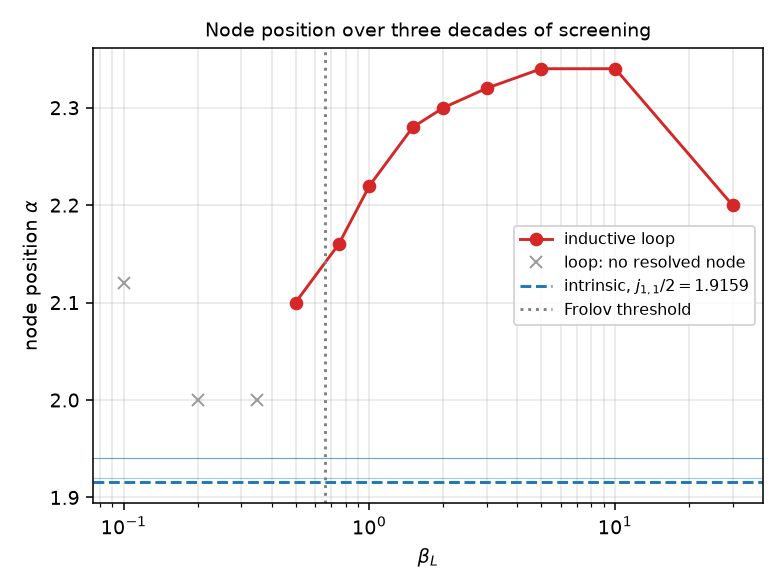
\includegraphics[width=\columnwidth]{figs/e4_floor_and_node.png}
  \caption{Node position against screening parameter over three decades, with
  the intrinsic node and Frolov's existence threshold marked. Crosses are
  settings where the loop's net half-step curve has no resolved minimum.}
  \label{fig:node}
\end{figure}

In the large-dc-current limit Tsarev and Fominov~\cite{Tsarev2025} give the
half-integer step amplitude as $\Delta j_{\pm n/2} = 2 j_2 |J_n(2\alpha)|$
[their Eq.~(39)], with their drive parameter equal to our $\alpha$. So
$w_{1/2}\propto|J_1(2\alpha)|$ and the first node sits at $2\alpha = j_{1,1}$,
i.e. $\alpha=1.9159$, independent of harmonic content. That is published and we
do not claim it; our numerics reproduce it, at $\alpha = 1.94$, $1.94$, $1.92$
for $c_2/c_1 = -0.15$, $-0.25$, $-0.40$, with node depths of
$5\times10^{-5}$ to $6\times10^{-4}$ against curve peaks of $0.055$ to $0.169$
--- three orders of magnitude.

What Eq.~(39) does not cover is the loop, which contains no CPR harmonic to be
proportional to. Table~\ref{tab:node} scans it over three decades.

\begin{table}[b]
  \caption{Loop node position against screening parameter, $a=0.3$. ``Resolved''
  means the net curve's minimum is at least five times below its peak. Frolov's
  existence threshold is $\beta_L = 0.659$.}
  \label{tab:node}
  \begin{ruledtabular}
  \begin{tabular}{cccc}
    $\beta_L$ & node $\alpha$ & miss vs $1.9159$ & resolved \\
    \colrule
    0.10 & 2.12 & $+10.7\%$ & no \\
    0.20 & 2.00 & $+4.4\%$  & no \\
    0.35 & 2.00 & $+4.4\%$  & no \\
    \colrule
    0.50 & 2.10 & $+9.6\%$  & yes \\
    0.75 & 2.16 & $+12.7\%$ & yes \\
    1.0  & 2.22 & $+15.9\%$ & yes \\
    2.0  & 2.30 & $+20.1\%$ & yes \\
    3.0  & 2.32 & $+21.1\%$ & yes \\
    5.0  & 2.34 & $+22.1\%$ & yes \\
    10   & 2.34 & $+22.1\%$ & yes \\
    30   & 2.20 & $+14.8\%$ & peak $7.6\times10^{-4}$ \\
  \end{tabular}
  \end{ruledtabular}
\end{table}

Three features matter, and only the first was visible in the three-point scan we
first ran. The miss \emph{saturates} at $\alpha=2.34$ from $\beta_L=5$ upward,
so the map from inductance to node position is not injective and cannot be
inverted to measure $\beta_L$ outside roughly one decade. Below Frolov's
threshold the miss falls to $+4.4\%$ --- consistent with Mori and Maekawa, whose
first-order-in-$\beta_L$ reduction puts the loop's node at $1.9159$ --- but
there the loop has no resolved node at all, the curve peaking at $0.002$--$0.008$
against $0.033$ at $\beta_L=2$. And by $\beta_L=30$ the half step has all but
died.

The usable statement is therefore bounded:

\begin{quote}
Within $\beta_L\in[0.66,10]$, where the inductive loop has a half step at all, a
node measured at $1.92$--$1.94$ is intrinsic and the loop misses it by $10$--$22\%$.
Outside that window the test does not apply --- below, because the loop has no
half step; above, because it has almost none.
\end{quote}

This is weaker than a parameter-free test, and we state it that way because an
earlier version of this work did not. The frequency test of
Sec.~\ref{sec:fails} died when its $\beta_L$ range was widened from a factor
$20$; this test was then built on a factor $4$, and widening it to three decades
is what produced Table~\ref{tab:node}.

\subsection{An aside on the two-order ratio}

The ratio $R_{23}=w_{\rm net}(\Omega/3)/w_{\rm net}(\Omega/2)$ is sometimes
called insensitive to drive calibration. In the voltage-biased limit it is not:
Duprat and Levy Yeyati's Eq.~(11)~\cite{Duprat2005} makes it
$|c_3J_1(6\alpha)|/|c_2J_1(4\alpha)|$, which passes through an exact node at
$\alpha=j_{1,1}/6=0.6386$. Under current bias the node disappears --- our scan
passes smoothly through it at $R_{23}\simeq0.185$ --- and the analytic reason is
in Ref.~\cite{Tsarev2025}, whose Eq.~(42) gives the third step as a \emph{sum}
of Bessel products rather than a single $J_1(6\alpha)$. The residual variation
is still $2.4\times$ over the accessible range, so ``insensitive'' overstates it.

\section{The flux axis separates the two extrinsic channels}

``Extrinsic'' is usually treated as one hypothesis. It is not. Moshe and
Mints~\cite{Moshe2007} treat a junction with spatially alternating critical
current density; their Eq.~(24) gives the half-step width at zero applied flux
as $v_1I_c(\gamma+\alpha^2)$ --- finite. We swept the inductive loop on the same
axis, $f\in[0,1]$ at $\beta_L\in\{0.5,2,10\}$ and $\Omega\in\{2,5,8\}$. At all
nine settings the net half-step width peaks at $f=0.50$--$0.60$ and sits at the
estimator floor at $f=0$: the loop's half step \emph{requires} frustration and
the alternating-$j_c$ channel's does not. That is the discriminator.

Two caveats belong with it. First, our $f=0$ point is the control that is
subtracted, so ``no step at integer flux'' is assumed there rather than
measured; the unsubtracted width at $f=0$ is $0.044$--$0.062$, which brackets the
independently measured sinusoidal floor of $0.050$--$0.060$, so the assumption
is consistent but not independent. Second, Moshe and Mints is voltage-biased and
perturbative while our loop is current-biased --- exactly the comparison that
failed for $R_{23}$ above. We therefore state the contrast on the half step
only, and do not extend it to the integer step: their Eq.~(25) makes $I_1$
vanish at $\phi_a=n\phi_0$ for $n\ge1$ but \emph{maximal} as $\phi_a\to0$, and
our loop's $w_1$ is likewise large at $f=0$. What is true in all nine of our
runs is that $w_1$ is \emph{minimal} near $f=0.50$--$0.60$.

\section{A systematic that prevents a thermal verdict}
\label{sec:thermal}

Two laws exist for how a fractional step of order $n/k$ survives thermal phase
noise: Duprat and Levy Yeyati's collapse against $k^2T$ at fixed
$k\alpha$~\cite{Duprat2005}, giving $\Gamma^*_k\propto k^{-2}$, and a barrier
estimate in which the relevant energy is the harmonic's own well depth
$|c_k|E_J$, giving $\Gamma^*_k\propto|c_k|$. The second is not a published law
but an estimate in common use, including in our own unpublished work; we name it
as such.

Separating them needs the $k$-dependence of the visibility threshold, and that
is where our method fails. Every width is net of a control, on the argument that
the control carries no fractional step so what it returns is the estimator's
transit floor, common to both and cancelling. It is not common: by
Eq.~\eqref{eq:kernel} the floor is $\sigma_k\sqrt{2\pi}/|dv/di|$, set by the
ohmic slope at the step, and the two CPRs do not share it. Measured at the
operating drives:

\begin{table}[b]
  \caption{Residual of the control subtraction at matched effective drive
  $k\alpha=2.4$. The bias is near-constant in magnitude while the net width falls
  $30\times$, so it lands on the $k$-dependence.}
  \label{tab:floor}
  \begin{ruledtabular}
  \begin{tabular}{ccccc}
    $k$ & $\alpha$ & net & bias & bias/net \\
    \colrule
    2 & 1.20 & 0.13329 & $-0.00198$ & $-1.5\%$ \\
    3 & 0.80 & 0.02173 & $-0.00350$ & $-16.1\%$ \\
    4 & 0.60 & 0.00461 & $-0.00271$ & $-58.7\%$ \\
  \end{tabular}
  \end{ruledtabular}
\end{table}

Restoring the measured bias moves the deterministic width ratio
$w_4/w_2$ from $0.0346$ to $0.0541$, a $56\%$ change. Survival is the ratio of
the noisy net width to its deterministic value, so $\Gamma^*$ inherits this
directly, and the statistical band --- which for us was $\pm0.0063$ on
$\Gamma^*_4/\Gamma^*_2=0.128$ --- does not cover it. We therefore report the
systematic and withhold the verdict. A measurement that would settle it needs
either an estimator whose floor does not depend on the transit slope, or a
control with the same slope as the signal.

We note what this does \emph{not} license. It does not establish either law; it
establishes that our measurement cannot separate them. An earlier version of
this work reported both as excluded, at $19.4\sigma$ and $6.0\sigma$. Those
numbers were percentile-band quotients from a $20{,}000$-draw Monte Carlo, which
resolves nothing past about $4\sigma$, and they omitted the systematic in
Table~\ref{tab:floor} entirely.

\section{What to measure}

For an experiment already producing a Shapiro map:
\begin{enumerate}
  \item \emph{Drive amplitude, through the node.} Compare the position with
        $1.9159$. Applicable when $\beta_L$ is plausibly in $[0.66,10]$; the
        loop then misses by $10$--$22\%$. The miss does not measure $\beta_L$.
  \item \emph{Trapped flux, over a full period.} A half step present at integer
        flux excludes the inductive loop; one present only near $f=1/2$ excludes
        the alternating-$j_c$ channel.
  \item \emph{Two drive frequencies.} An increase in $w_{1/2}/w_1$ below $56\%$
        from $\Omega=2$ to $8$ excludes the intrinsic mechanism. A larger rise
        decides nothing.
\end{enumerate}
None requires thermal cycling, field training or current annealing. None
replaces them: all three are one-sided, and the first is conditional on a
parameter the experiment does not independently know.

\section{Limitations}

The extrinsic mechanism is one caricature; a spatial $I_c$ distribution, a
series chain, or phase-slip centres may behave differently. The frame is
overdamped, $\beta_c\simeq0$ --- and Ref.~\cite{Tsarev2025} Sec.~6 notes that
finite capacitance generates a full devil's staircase of subharmonic steps from
a \emph{sinusoidal} CPR, so for an underdamped junction the two-hypothesis
framing of this paper is not exhaustive. Cuprate junctions may well be
underdamped. The node and flux scans are noiseless, and finite temperature could
shift a node. The asymmetry $a=0.3$ is fixed throughout and the node's
dependence on it, and on $f$, is untested. Section~\ref{sec:fails}'s numbers
carry the grid-counting systematic noted in Sec.~II.

\begin{acknowledgments}
Every figure and table here is produced by a script committed alongside this
work, against data artifacts committed with it.
\end{acknowledgments}

\begin{thebibliography}{9}

\bibitem{Zhu2026}
  Y.~Zhu, H.~Wang, D.~Zhang, and Q.-K.~Xue,
  \emph{Manipulating fractional Shapiro steps in twisted cuprate Josephson
  junctions},
  \href{https://arxiv.org/abs/2512.01586}{arXiv:2512.01586}.

\bibitem{Early1994}
  E.~A.~Early, R.~L.~Steiner, A.~F.~Clark, and K.~Char,
  Phys.\ Rev.\ B \textbf{50}, 9409 (1994).

\bibitem{Terpstra1995}
  D.~Terpstra, R.~P.~J.~IJsselsteijn, and H.~Rogalla,
  Appl.\ Phys.\ Lett.\ \textbf{66}, 2286 (1995).

\bibitem{Tsarev2025}
  P.~N.~Tsarev and Y.~V.~Fominov,
  SciPost Phys.\ \textbf{19}, 148 (2025),
  \href{https://arxiv.org/abs/2505.20502}{arXiv:2505.20502}.

\bibitem{Beenakker1991}
  C.~W.~J.~Beenakker,
  Phys.\ Rev.\ Lett.\ \textbf{67}, 3836 (1991).

\bibitem{Frolov2006}
  S.~M.~Frolov, D.~J.~Van~Harlingen, V.~V.~Bolginov, V.~A.~Oboznov, and
  V.~V.~Ryazanov,
  Phys.\ Rev.\ B \textbf{74}, 020503(R) (2006).

\bibitem{Mori2021}
  M.~Mori and S.~Maekawa,
  Appl.\ Phys.\ Express \textbf{14}, 103001 (2021),
  \href{https://arxiv.org/abs/2108.11006}{arXiv:2108.11006}.

\bibitem{Duprat2005}
  R.~Duprat and A.~Levy~Yeyati,
  Phys.\ Rev.\ B \textbf{71}, 054510 (2005).

\bibitem{Moshe2007}
  M.~Moshe and R.~G.~Mints,
  \href{https://arxiv.org/abs/0708.1222}{arXiv:0708.1222} (2007).

\end{thebibliography}

\end{document}
